\documentclass[]{elsarticle} %review=doublespace preprint=single 5p=2 column
%%% Begin My package additions %%%%%%%%%%%%%%%%%%%
\usepackage[hyphens]{url}
\usepackage{lineno} % add
\providecommand{\tightlist}{%
  \setlength{\itemsep}{0pt}\setlength{\parskip}{0pt}}

\bibliographystyle{elsarticle-harv}
\biboptions{sort&compress} % For natbib
\usepackage{graphicx}
\usepackage{booktabs} % book-quality tables
%% Redefines the elsarticle footer
%\makeatletter
%\def\ps@pprintTitle{%
% \let\@oddhead\@empty
% \let\@evenhead\@empty
% \def\@oddfoot{\it \hfill\today}%
% \let\@evenfoot\@oddfoot}
%\makeatother

% A modified page layout
\textwidth 6.75in
\oddsidemargin -0.15in
\evensidemargin -0.15in
\textheight 9in
\topmargin -0.5in
%%%%%%%%%%%%%%%% end my additions to header

\usepackage[T1]{fontenc}
\usepackage{lmodern}
\usepackage{amssymb,amsmath}
\usepackage{ifxetex,ifluatex}
\usepackage{fixltx2e} % provides \textsubscript
% use upquote if available, for straight quotes in verbatim environments
\IfFileExists{upquote.sty}{\usepackage{upquote}}{}
\ifnum 0\ifxetex 1\fi\ifluatex 1\fi=0 % if pdftex
  \usepackage[utf8]{inputenc}
\else % if luatex or xelatex
  \usepackage{fontspec}
  \ifxetex
    \usepackage{xltxtra,xunicode}
  \fi
  \defaultfontfeatures{Mapping=tex-text,Scale=MatchLowercase}
  \newcommand{\euro}{€}
\fi
% use microtype if available
\IfFileExists{microtype.sty}{\usepackage{microtype}}{}
\usepackage{graphicx}
% We will generate all images so they have a width \maxwidth. This means
% that they will get their normal width if they fit onto the page, but
% are scaled down if they would overflow the margins.
\makeatletter
\def\maxwidth{\ifdim\Gin@nat@width>\linewidth\linewidth
\else\Gin@nat@width\fi}
\makeatother
\let\Oldincludegraphics\includegraphics
\renewcommand{\includegraphics}[1]{\Oldincludegraphics[width=\maxwidth]{#1}}
\ifxetex
  \usepackage[setpagesize=false, % page size defined by xetex
              unicode=false, % unicode breaks when used with xetex
              xetex]{hyperref}
\else
  \usepackage[unicode=true]{hyperref}
\fi
\hypersetup{breaklinks=true,
            bookmarks=true,
            pdfauthor={},
            pdftitle={Predictive Models to Support Quoting of Fixed Fee Consulting Projects},
            colorlinks=true,
            urlcolor=blue,
            linkcolor=magenta,
            pdfborder={0 0 0}}
\urlstyle{same}  % don't use monospace font for urls
\setlength{\parindent}{0pt}
\setlength{\parskip}{6pt plus 2pt minus 1pt}
\setlength{\emergencystretch}{3em}  % prevent overfull lines
\setcounter{secnumdepth}{0}
% Pandoc toggle for numbering sections (defaults to be off)
\setcounter{secnumdepth}{0}
% Pandoc header


\usepackage[nomarkers]{endfloat}

\begin{document}
\begin{frontmatter}

  \title{Predictive Models to Support Quoting of Fixed Fee Consulting Projects}
    \author[Queensland University of Technology]{Amy Cook, Paul Wu, Kerrie Mengersen\corref{c1}}
   \ead{a21.cook@qut.edu.au} 
   \cortext[c1]{Corresponding Author}
      \address[Queensland University of Technology]{School of Mathematical Sciences, George Street, Brisbane, QLD, 4000}
  
  \begin{abstract}
  A concise abstract is required. limit to 250 words. clearly state
  purpose of research, principal resutls and major conclusions. no refs
  
  Engaging in loss making jobs for fixed fees is a major problem in
  consulting, particularly in the competitive construction industry. This
  thesis investigates whether machine learning techniques applied to a
  company's passively collected internal data could help avoid loss making
  jobs or help tactfully choose when to enforce stricter contracts. It was
  found that in a specific decision framework, a case study's profits
  could be improved 9\% by declining approximately 4\% of projects.
  Alternative decision frameworks are also proposed and evaluated.
  Algorithmic methods such as Logistic Regression, Random Forests, Boosted
  Trees, Naive Bayes, and Bayesian Networks were applied as well as
  blended combinations of these methods. A decision scenario which
  rejected projects above a sequence of tested thresholds was run in order
  to find the optimal threshold for profit improvements. The blended
  Logistic Regression model outperformed other methods and produced a 95\%
  confidence interval of 6.5 - 11.5\% profit improvements. The findings
  from this research have the potential to assist managers in reducing
  losses by highlighting risky projects and guiding project-based changes
  to fee structures.
  \end{abstract}
   \begin{keyword} consulting; machine learning; profitability; predictive model;
construction industry; data mining \sep \end{keyword}
 \end{frontmatter}

\emph{Text based on elsarticle sample manuscript, see
\url{http://www.elsevier.com/author-schemas/latex-instructions\#elsarticle}}

\section{1. Introduction}\label{introduction}

Clearly state the research question and objectives of the work. Briefly
provide any necessary background to frame the research question.
Concisely summarize the major findings/results.

Many consulting projects can be financialy risky endeavors for the
consultant, often depending on the industry. Engineering consultanting
companies in the construction industry complete a wide range of complex
projects in a competitive enviroment. Because of the way contracts are
structured, many of these projects result in losses. The purpose of this
study was to test whether these loss making projects could be predicted
by statistical and machine learning algorithms using the information
available at project conception. Secondly, could the predictive
algorithm improve a company's profitability? Predictive models and value
frameworks were built using project data from a case study engineering
company to answer these questions.

1 page

\paragraph{1.1 Problem motivation}\label{problem-motivation}

Financial risk is taken on by a consulting company when they offer a
fixed fee to complete a project. In competitive climates, clients are in
the position to request fixed price quotes from several consultants
before a project is awarded. Hence, initial quoted fees must be
competitive but also accurately cover consultant salaries and business
costs.

How do consultants make this accurate yet competitive fee estimate? This
varies from industry to industry, but typically a consulting manager has
experience in the type of project they are quoting and, after reviewing
the project details, can use a combination of intuition, analysis of
project details, and rules of thumb. Unfortunately, some projects priced
using this method can blow out of budget, causing significant financial
losses to the consultant.

Cost blowouts of complex projects has a history, particularly documented
in the It and construction industry. A review of 6 IT project surveys
between 1984 and 1994 by Moløkken \& Jørgensen (2003) revealed that
60-80\% of IT projects encountered effort and/or schedule overruns,
where the average overrun was by 30 to 40\%. A study on large-scale
infrastructure projects over the past seventy years revealed that cost
forecasts consistently underestimated the cost of rail projects by an
average of 44.7\%, the cost of bridge and tunnel projects by 33.8\% and
the cost of road projects by 20.4\% (Flyvbjerg 2007).

Kahneman won a nobel prize in 2002 for his research into decision making
on this topic. He argued that a person's natural optimistic view of
their own skills leads to consistent underestimation of the time and
risks involved in a project (Lovallo and Kahneman 2003). To counter this
phenomenon, research by Flyvbjerg {[}-Flyvbjerg2011{]} advised that
managers should be confronted by the financial performance of similar
projects to the one being costed so that they take on a more realistic
view of their abilities. This was based off a body of findings where
people made better predictions about themselves after being exposed to
facts about other people. For example, subjects were asked to predict
their skill levels before and after being exposed to a summary of other
people's skills, and their predictions after were significantly more
accurate (Lovallo and Kahneman 2003).

This work aims to help managers provide better fixed price quotes by
predicting whether a new project will be profitable or not, based on an
algorithm trained on all previous project data from the same company.
The manager could take multiple actions based on the algorithms output
including not tendering for a project predicted to be loss-making,
providing a high fixed price, or restructuring the contract so that it
is not 100\% fixed price. This research tests the simple case of
rejecting all projects predicted as loss-making.

\paragraph{1.2 Case Study}\label{case-study}

Project data from a single case study consulting company in the
construction industry was used to build the predictive algorithm, trial
several methods, and test their impact on the company's bottom line.
Twelve years of passively collected data that described each project in
terms of their clients, invoice history, employee hours and technical
details was scraped from the company's internal database. Customer
relationship management (CRM) software provided accesses to the database
to all employees. Employees completed daily timesheets, alotting their
hours to certian projects. Project managers input technical information
and client details for each project, while the finance team tracked
invoicing and additional project costs such as printing and transport in
the same system. On top of this information, the CRM had the hourly cost
of each level of employee. The cleaned dataset consisted of 2364
projects between 2004 and 2012. 70\% of projects were fixed price and
20\% of all projects made a loss after taking into account business
costs.

Once several methods were built, to assess whether the model would
improve the case study company's profitability, a simple managerial
decision framework was applied: if the algorithm predicted the project
to be loss making, the project was considered `rejected' and all profits
or \emph{losses} of rejected projects were discarded. The remaining
projects' profits and losses were summed to give a revised overall
profit over the last 12 years of projects. This was compared to the
summed profits and losses from all projects completed over the last 12
years. The best algorithm rejected enough loss-making projects to
improve overall profits by 9\%.

\section{2. Literature Review}\label{literature-review}

For the case study company, training the algorithm to predict actual fee
was not possible because the projects were too varied, and there was
inadequate information describing the size and scope of each project in
the database. However, in the literature, similar studies typically did
attempmt to predict project costs of IT consutling projects and final
construction costs of buildings and infrastructure.

\paragraph{2.1 Cost estimation in the Construction Industry and IT
Industry}\label{cost-estimation-in-the-construction-industry-and-it-industry}

Previous studies in the literature have focussed on reporting the
predictive accuracy of their cost estimation models for IT or
construction projects using data from multiple businesses or governments
around the world. In contrast, this research is focussed on determining
how or if models predicting project profitability can improve the bottom
line for a case study business, given data the company has internally
generated.

Reviewing a range of individual studies show that cost estimation models
have generally been built from at most 530 projects (Kim, An, and Kang
2004) (Finnie, Wittig, and Desharnais 1997) - 299 software
development(Pai, McFall, and Subramanian 2013) - 163 software (Shin
2015) - 234 building projects, and often under 100 projects (Finnie,
Wittig, and Desharnais 1997) (Chan and Park 2005) 87 buildings.
Sometimes it is not stated where the project data came from, and some
studies specified the information came from surveys, with responses from
companies and governments around the world. In this study, the dataset
originates from a single company's database, which means the data is
easily accessible to the company and there are 2364 projects, which is
much more than previous studies. A study by Mendes and Kitchenham (2004)
demonstrated that using within company data was also more accurate than
across company data. Their dataset consisted of 67 across company web
projects and 14 within company projects.

Almost all past studies analysed their model performance by predictive
accuracy (reported as R\^{}2 or RMSE) of cost predictions
({\textbf{???}} some stff) and compared these statistics bewteen
methods. However, these results were not translated into a business case
for the impact these models could have on an institution or how the
model could be practically integrated into decision making. For example,
if an institution used the model, how would it be applied to their
decision making process and what magnitude of benefits could they
expect? Saradhi \& Palshikar's (2011) work on employee churn, where
`churn' refers to the number of individuals moving out of a group within
a certain time, presented a good framework for implementing their model.
Theirsupport vector machine (SVM) predictive model identified employees
at high risk of churn. Then a method for determining the value of each
employee in terms of their importance to projects and their monthly
chargeability was described, which enabled high risk employees to be
ranked. Managers then had a clear direction for who to target first to
prevent churn. This extension provided a comprehensive framework for how
business managers could adopt a machine learning algorithm to improve
business operations. It was a valuable addition that is absent from most
cost estimation research, but will be included in this work.

\paragraph{2.2 Methods used in Cost Estimation and Other Business
Applications}\label{methods-used-in-cost-estimation-and-other-business-applications}

Cost estimation literature tended to apply linear regression, neural
networks and sometimes SVM methods, while predictive methods applied to
other business problems investigated a wider range. This study aims to
compare a wider range of methods to past cost estimation studies.

In the construction industry, often only one method was assessed, such
as linear regression, without comparison to other methods (Chan and Park
2005; Elfaki, Alatawi, and Abushandi 2014). Neural Networks started
appearing in literature in the 1990's and Elfaki, Alatawi, and Abushandi
(2014)`s review of cost estimation methods from 2004 to 2014 found that
artificial Neural Networks and SVM's were the most popular machine
learning techniques, but studies tended to only test one method. Some
studies showed that Neural Networks outperformed Linear Regression,
however other studies established they are approximately equal (Kim, An,
and Kang 2004; Attalla and Hegazy 2003). To the authors' knowledge Shin
(2015) documented the only application of ensemble tree methods (Boosted
Trees) to cost estimation in construction projects. They found Boosted
Trees slightly outperformed Neural Networks, but not significanatly.

In the software cost estimation literature, Linear Regression was the
most popular method, however multiple studies showed that Neural
Networks definitively outperform regression models (Finnie, Wittig, and
Desharnais 1997; Pai, McFall, and Subramanian 2013; Matson and
Mellichamp 1993). Despite the higher performance, Neural Networks were
criticised for not providing reasoning or structure behind their
predictions (black-box predictor) (Finnie, Wittig, and Desharnais 1997).

The review of methods applied to the construction and IT industry
highlighted the use of Linear Regression, Neural Networks, SVM's and in
one case Boosted Trees, however research on other business problems
utilised a wider range of methods. In financial credit scoring, a study
by Brown and Mues (2012) found that Random Forests and Boosted Trees
consistently outperformed Neural Networks in classification. In
addition, ensemble trees such as Random Forests and Boosted Trees can
output partial dependency plots and variable importance measures that
provide insight into the model's calculations. This is a valuable asset
oer black box predictors. Kumar and Ravi (2007) performed a detailed
review of statistical and machine learning techniques applied over 37
years in the context of bankruptcy prediction in banks and reported that
although SVM's performed well, they are often complex and slow,
requiring a great deal of memory. They also assessed method blending
techniques, which refers to combinations of two completely different
algorithms, and found they can often outperform individual methods such
as Linear Regression or Boosted Trees alone.

To date, Linear Regression, Neural Networks, and Support Vector Machines
(SVM's) have been comprehensively applied to cost estimation. This
research does not test black-box predictors (Neural Networks and SVM's)
because insight into the model's predictions is crucial for facilitating
user uptake in the case study company. Ensemble tree methods such as
Random Forests and Boosted Trees will be used instead, as they can
perform as well as Neural Networks while providing insight to their
output (Caruana and Niculescu-Mizil 2006). Blending of multiple
predictive models is also applied in this work and has not yet been done
in cost estimation.

\paragraph{2.3 Gaps}\label{gaps}

In comparison to previous studies, this project advances the body of
work on cost estimation in two ways. First, it focusses on building a
model that is practical and profitable for a business to implement by
using the case study's interenal database as well as testing a
managerial decision framework based off the model output. This framework
presents a clear measure of expected benefits provided by adopting the
profitability model into a business' decision process. Secondly,
advanced predictive methods are trialled which have been minimally
tested on this problem. These include ensemble decision tree methods,
such as Random Forests and Boosted Trees, and blends of multiple models
built from different methods.

\section{3. Prediction Methods}\label{prediction-methods}

Should provide sufficient detail to allow the work to be reproduced.
Methods already published should be indicated by a reference: only
relevant method modifications should be described.

Neural Netowrks and SVM were not purusued because black box A previously
mentioned disadvantage is that the NN algorithm is a black box because
the internal structure is too complex for interpretation. They also
require a lot of training data relative to other methods.

Also, SVM's can be very slow to train and therefore not suitable for
industry purposes (Auria and Moro 2008). Because it is so important to
engage decision makers with a model that can explain its results, these
two methods are not appropriate for the effort estimation problem.

\paragraph{3.1 Predictive methods}\label{predictive-methods}

binary classification problems, where the objective is to predict the
probability of an event occurring. Probability is a continuous response
variable, however predictions from a linear regression would not be
bound by 0 and 1.

\subparagraph{3.1.1 Logistic Regression}\label{logistic-regression}

Because of the linear relationship, an equation can be fit to the log
odds of the binary response variable against each of the explanatory
variables using linear regression. Then, the linear equation describing
the log odds can be transformed back to probability by taking the
inverse log i.e.~the exponential and rearranging (Macdonald 1975):

The result in a sigmoidal function bound by 0 and 1. The sigmoidal
function originates from a linear fit of the log odds in the data.
Assume linear relationship between covariates and response variable

A coefficient represents the change in the log odds of the response
variable for each unit increase in an explanatory variable. Therefore,
taking the exponential of the coefficient is the change in odds of the
response variable. If the change in odds was 2, then if the explanatory
variable increased by 1, the response variable event would be twice as
likely to occur.

Logistic Regression is a good benchmark to compare other binary
predictive models due to its simplicity and speed (Moore and McCabe
1989). single linear relationship means Not prone to overfitting

\subparagraph{3.1.2 Random Forests}\label{random-forests}

single decision trees also suffer from low predictive accuracy and
instability, so to combat these problems, ensemble tree methods were
pioneered in the 1990's (Breiman 1996).

The three methods of combining hundreds or thousands of trees turn
decision trees into high performing, stable predictors.

training multiple trees from the same data by sampling bootstrapped
training sets with replacement. However, when creating each tree, a
random subset of attributes (variables) is considered at each split. The
reduced subset of attributes is resampled for each split in the tree.
This allows dominant variables to be suppressed for a fraction of the
splits, allowing the algorithm to explore signals in weaker variables
(Breiman 2001).

Additionally, ensemble tree methods are faster than SVM's and Neural
Networks but can perform just as well and even provide insights such as
variable importance and variable relationships (Sealfon and Gymrek
2012).

\subparagraph{3.1.3 Gradient Boosted
Trees}\label{gradient-boosted-trees}

Lastly, the boosted decision tree approach applies gradient descent
theory to a series of decision trees. The trees are limited to a certain
depth to maintain simplicity, and each tree models the residuals (or
errors) of the preceding tree. By modeling the errors, misclassified
cases are weighted higher than correctly classified cases and influence
the structure of the latest tree more (Hastie, Tibshirani, and Friedman
2009). This increased weighting on errors is why the algorithm is called
boosting. The limited depth of each tree prevents overfitting at each
stage and the combined result of up to thousands of trees is very
powerful (Elith, Leathwick, and Hastie 2008).

Caruana and Niculescu-Mizil (2006) tested Boosted Trees, Random Forests,
Neural Networks, SVM's, Logistic Regression and Naive Bayes on 11 binary
classification problems and found that Boosted Trees performed best,
followed by Random Forests. This demonstrates how ensemble tree methods
are capable of competing with high-level machine learning algorithms.

Trees are not built on a probabilistic framework, and therefore their
results cannot be provided in this framework (Louppe and Prettenhofer
2014).

\subparagraph{3.1.4 Naive Bayes}\label{naive-bayes}

The Naive Bayes method works by making conditional independence
assumptions about the explanatory variables in order to simplify
probability calculations for the response variable (the response
variable must be categorical).

These equations are simple to compute given the data, and the class with
the highest probability can then be chosen (F. Provost and Fawcett
2013).

The advantages of this method are that the conditional independence
assumption enables very fast calculations and predictions. The method
can perform well in real world tasks because the assumption of
independence does not significantly damage predictions (F. Provost and
Fawcett 2013). Assumptions of independence genearlly not true
(correlated variables). This is fine for ranking but the output
probabilities are not accurate statistical probabilities (Caruana and
Niculescu-Mizil 2006).

Naive Bayes method generally provides a good benchmark to compare
against more complex models that should outperform it (Caruana and
Niculescu-Mizil 2006).

\subparagraph{3.1.5 Bayesian Networks}\label{bayesian-networks}

A Bayesian Network is a graphical probabilistic model that illustrates
the conditional dependencies between variables in a data set. The model
is visually represented by a directed acyclic graph (DAG) and is capable
of linking the conditional dependency between any variable to another
variable (Heckerman 1998). The conditional relationships are Bayesian,
where the probabilities in one node are conditional upon values in nodes
directed towards it as well as preceding nodes

Bayesian Networks reduce computations required to find the probability
of a unique combination given other explanatory variable values while
still taking into account many conditional dependencies that Naive Bayes
(Barber 2012)

Naive Bayes is the simplest form of a Bayesian Network (Zhang 2004)

Network relationships can be learned from the data, however this is not
widely included as part of the suite of machine learning methods. The
conditional variable dependencies are calculated from the data, which in
turn can define the graph structure. Some conditional dependencies can
be set before the structure is learned (Barber 2012).

Drawbacks of Bayesian Networks include the difficulty for them to
process continuous variables.

Bayesian networks have found success in combining deterministic models
with observed data as well as expert knowledge.(Kragt 2009)

\paragraph{3.2 Procedure}\label{procedure}

It includes first how the data was obtained, the lengthy cleaning
process, Projects varied from total invoiced amounts of \$500 to over
\$1,000,000 a project could have thousands of rows of relevant data that
needed to be converted into a single row per project. 10 engineered
variables describing timesheets: Percent of hours performed by
`professional' employees as opposed to `technical' employees, Position
of the employee that completed the most hours on each project 3
engineered from invoicing data: 4 from project data: number of projects
completed with each client text analysis of project titles to develop
project classifications

Discretisation was performed by generating a hierarchical dendrogram of
each variable to visualise the clusters.

Limiting the predictive model to a concise set of meaningful variables
reduces noise and improves predictions. Less variables and a simpler
model is easier for stakeholders to understand (Weisberg 2005). followed
by variable importance analysis, variable selection: varialbe importance
aalyses done with linear regression, random forest, cforest to represent
the range of algroithms that were trialled. 11 variables chosen:

trials of selected predictive algorithms. binary classification problem
predicting profit or loss. Complex models should be measured against
simple models that can be built at a fraction of the computational cost.

\begin{itemize}
\tightlist
\item
  Regression - baseline model
\item
  Naive Bayes - baseline model
\item
  Bayesian Network - grabage.
\item
  Random Forest
\item
  Gradient Boosted Trees
\end{itemize}

To compare the models, the area under the receiver operating
characteristic (ROC) curve (AUC) statistic was used. An ROC graph
visualises the curve from which an AUC score is calculated. In this
problem a `positive' is a loss making job. For binary classification,
AUC is a more meaningful statistic than classification accuracy when the
output is a probability that can be applied to the problem. The AUC
indicates model performance across many thresholds while classification
accuracy represents a single threshold.

a model must be first created using a training set. The model can then
make predictions on the test set. this is used to build the ROC A model
that is perfectly classified would have an AUC = 1. A model that
predicts as well as random chance would have an AUC = 0.5. An AUC
between 0.5 and 1 means the model is performing better than random
chance.

In order to compare which models performed significantly better than
others, an adequate sample size of results statistics is required.
Multiple models could be made by using different data in the training
vs.~testing sets, each providing a resulting test statistic (RMSE or
AUC). Initially, 20 models of each method were created in this fashion.
Then a two-sample power calculation was run using the two sets of 20
results to determine the sample size to achieve a statistical power of
0.8 (100 to achieve power of 0.8 between boosted trees and naive bayes)

Missing Data Imputation. All methods except gradient Boosted Trees and
Naive Bayes could not handle missing data. a complete data set allows
for complete sets of predictions from each method, and these predictions
could then be blended to further improve results. The MICE Random Forest
method was chosen for imputation because it has been proven to work well
with complex data sets (Shah et al. 2014). If similar predictive results
were obtained using Boosted Trees imputed data and imputed data, the
imputed data must be reasonable. The imputed data set was then trialed
on the remaining methods and compared to unimputed trials.

Once the best methods were selected, they were blended in numerous ways,
using both simple averaging techniques and sophisticated
machine-learning algorithms. These were compared against individual
models and the best constructs were selected. Six blending methods,
ranging from simple to complex, were tested using predictions from the
top performing individual models. These included simple averaging of the
individual model results, building a Logistic Regression model using the
individual model results only, a Boosted Tree model using individual
model results only, feature weighted linear stacking (FWLS), Random
Forests, and Boosted Trees. A simplified explanation of FWLS is as a
Linear Regression where meta-features as well as model predictions from
individual models are included as explanatory variables. Then, each
meta-feature is interacted with each set of model results (Sill et al.
2009). Feature interaction is performed passively due to the nature of
how trees are built. A split in a node determined by one variable is
conditional upon the preceding split, which was based on another
variable and so on. The simplest method averaged the probability output
(a number between 0 and 1) of all three models. The next two simplest
methods consisted of building a Logistic Regression and Boosted Trees
model from the three prediction model outputs only. Feature Weighted
Linear Stacking (FWLS), Random Forest and Boosted Trees were also tested
as blending methods in a more complex scenario where the predictions
from each model became additional variables to the original explanatory
variables (called meta-features in this context). The model predictions
were interacted with each original variable so that models that
performed more strongly under certain meta-feature states could be
weighted as such.

Again, 100 models were built to achieve a power of 0.8 for the variation
in AUC test statistics across different divisions of training/testing
data. A maximum of five blended models were created from a complete set
of test results (built from the individual models), then a new set of
test results were created for the next five blended models.

Finally the impact of the algorithm on the overall profits of the case
study company was analysed via decision-making scenarios. This analysis
differed from accuracy in predicting profitability, so several blended
models as well as individual models were carried forward for this
analysis. This was done using a profit curve - a chart that plots the
change in profit the company earns on the y-axis vs.~the probability
threshold on the x-axis. A simple approach was taken for this analysis,
where projects with a probability to be a loss making job greater than
the threshold were rejected entirely. Therefore all profits and losses
from jobs above the threshold were discounted. An equation defining the
change in profit as a percentage of the original profit using threshold
rejection is shown below:

\begin{equation}
\Delta\ Overall\ Profit\ \textrm{(\%)} = \frac{\sum_{p = 1}^{N} I(Pr_p < threshold) \cdot Profit_p}{\sum_{p = 1}^{N} Profit_p} \cdot100
\end{equation}

Where

\[
\begin{aligned}
I(\cdot) &= \textrm{the indicator function} \\
N\ &= \textrm{the number of individual projects that are being included in the analysis} \\
Pr_{p} &= \textrm{probability output from the algorithm for project}\ p \textrm{. Values are}\\
& \qquad \textrm{betweeen 0 and 1 where 1 is loss making)} \\
threshold &= \textrm{a chosen value between 0 and 1.}\ \Delta\ Overall\ Profit\ \textrm{is calculated for} \\
& \qquad \textrm{several}\ threshold\ \textrm{values which defines the profit curve} \\
Profit_p &= \textrm{profit for individual project}\ p
\end{aligned}
\]

If the threshold was zero, all jobs were rejected and the profit would
be \$0. If the threshold was 1.0, all jobs were accepted and the profit
would be the same as the profit the company actually experienced since
the data is a sample of historic projects. The aim was to find the
optimal threshold point where saying `no' to a job above that level
would result in higher profits, because jobs that were likely to make a
loss were being rejected. This chart will clarify what percentage of
profit increase the company could expect by integrating the algorithm
into decision-making.

the curve varies with different divisions of the data. Therefore, in
order to understand the uncertainty around the profit curve and to
determine which blended or individual model performed statistically
better than others, a large sample size of curves was required. 100 to
achieve a power of 0.8. which was achieved by repeating 5-fold
training/testing splits. A 95\% confidence interval could also be
determined around the highest point on each curve. The final expected
increase in profit and the percentage of projects to be rejected
presented a clear scenario that the case study business managers could
assess in terms of their business strategy.

\section{4. Prediction Results and
Discussion}\label{prediction-results-and-discussion}

Present results clearly and concisely discussion should explore the
signficance of the results of the work, not repeat them.

\paragraph{4.1 Individual Models}\label{individual-models}

The predictive formula was re-structured so that the 11 explanatory
variables predicted a new response variable: profitable/unprofitable
projects. The five prediction methods, were initially built without
imputing data, by using the maximum amount of data possible depending on
the method. Boosted Trees and Naive Bayes are able to process data with
missing values, so all data could be input (Ridgeway 2015; Meyer et al.
2014). 100 models of each method were built. The violin plot below
summarises the AUC values produced by each method and the `violins' are
coloured according to whether the distributions significantly vary to
Boosted Trees using a critical value of 0.05.

\begin{figure}[htbp]
\centering
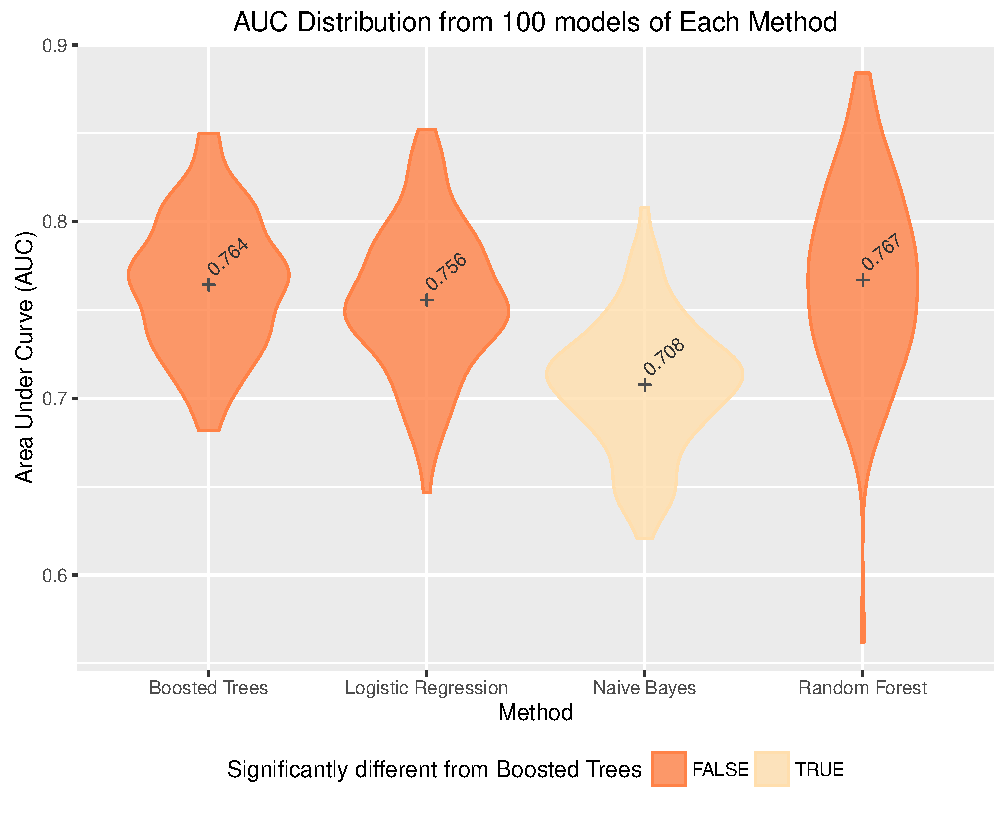
\includegraphics{Consulting_Profitability_Paper_files/figure-latex/reduced_violin-1.pdf}
\caption{Violin plot vertically illustrating the distribution of AUC
values from each of the methods when predicting profit/loss. Subsets of
the data were used for Logistic Regression and Random Forests in order
to provide datasets without missing values.}
\end{figure}

The AUC performance of Logistic Regression and the Random Forest
algorithms cannot be statistically differentiated from Boosted Trees.

Next, data imputation methods were trialed which would make the complete
data set available to Logistic Regression and Random Forests. Again, 100
models were required to achieve a power of 0.8 with respect to Boosted
Trees

\begin{figure}[htbp]
\centering
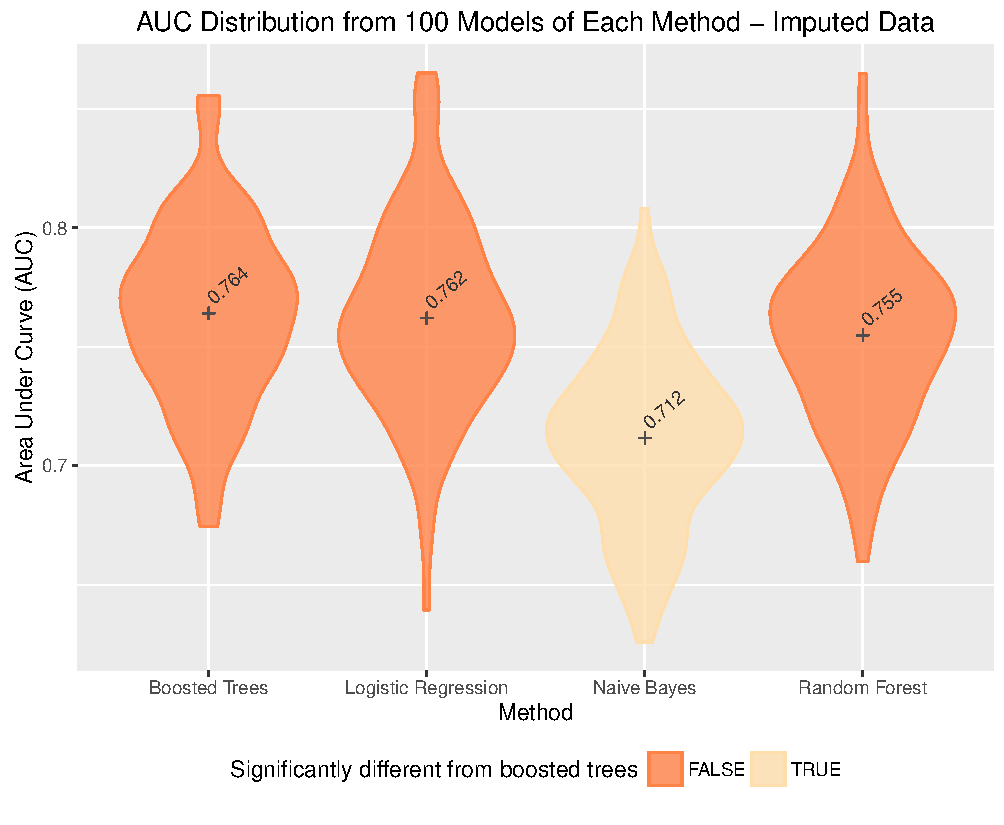
\includegraphics{Consulting_Profitability_Paper_files/figure-latex/mice_violin-1.pdf}
\caption{Violin plot vertically illustrating the distribution of AUC
values from each of the methods when predicting profit/loss. Each method
was fed the same imputed full dataset.}
\end{figure}

Boosted Trees, Logistic Regression, and Random Forest all performed
significantly better than the baseline algorithm, Naive Bayes, however
none outperformed Boosted Trees.

Testing Boosted Trees, Random Forests, Naive Bayes, Logistic Regression
and Bayesian Networks on the binary classification problem showed that
Boosted Trees, Logistic Regression and Random Forests performed best
(according to AUC). Naive Bayes and Logistic Regression were included as
baseline models and it was expected that the more complex models would
outperform these. Therefore it was surprising that results from 100
Logistic Regression models were not statistically significantly lower
than Boosted Trees.

A possible explanation for this, according to the literature, is that
there was not enough data for the ensemble trees to learn the complex
decision rules at which they excel. Trees tend to overfit the patterns
in a smaller training set. Logistic Regression on the other hand is
capable of only one decision boundary (which does not have to be
parallel to the variable axes) and is not prone to overfitting (Perlich,
Provost, and Simonoff 2003). This may explain Logistic Regression's
comparatively high performance on the case study's small but complex
data set.

Boosted trees, Random Forests and Logistic Regression all had mean AUC
values between 0.755 to 0.764. In summary, the individual binary
classification models performed well above random chance (AUC = 0.5).
Whether the model is worth implementing in the work place is dependent
on the extent to which the algorithm would improve `bottom line' profits
for the business and if the model can affect decisions in practice.

\begin{itemize}
\tightlist
\item
  NB and BN were bad - one sentence
\end{itemize}

\paragraph{4.2 Blended Models}\label{blended-models}

Blended models combine the predictions from each high-performing
individual model to create averaged or `blended' predictions. In this
case, the Random Forest, Boosted Trees, and Logistic Regression models
were chosen. Through variable importance studies, 6 variables were
included as metafeatures. All six methods were compared against the
original Logistic Regression model's AUC distribution (as it was not
statistically different from the ensemble trees)

\begin{figure}[htbp]
\centering
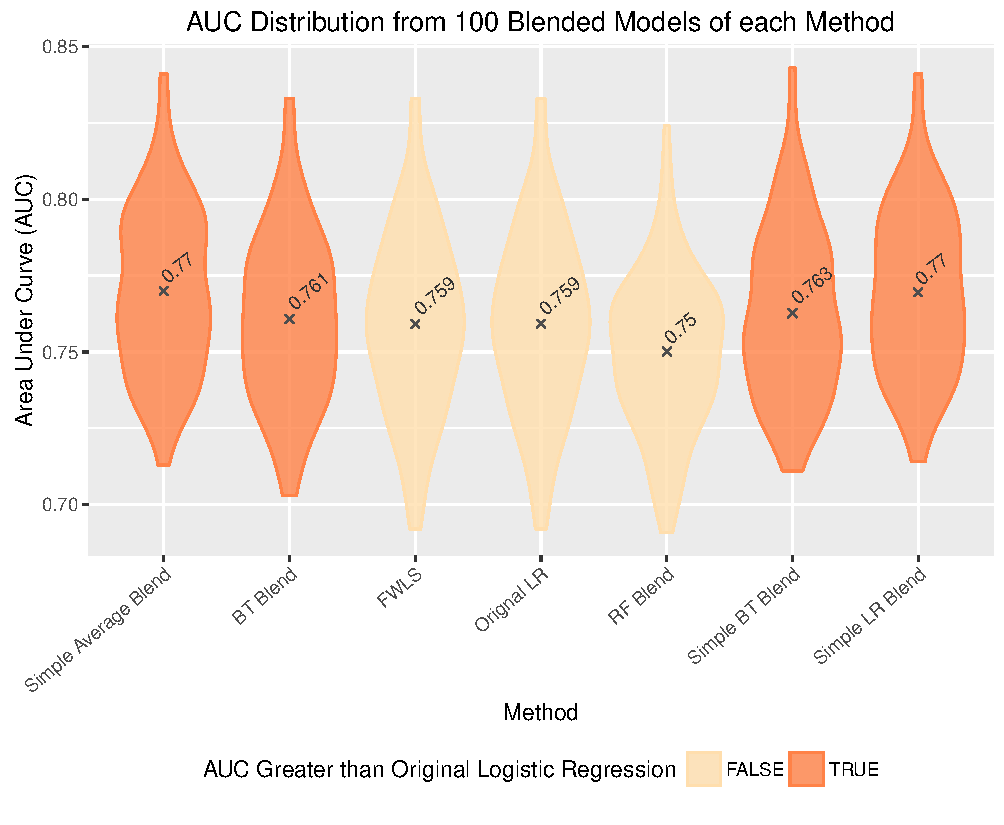
\includegraphics{Consulting_Profitability_Paper_files/figure-latex/blend_violin-1.pdf}
\caption{Violin plot vertically illustrating the distribution of AUC
values from each of the blending methods when predicting profit/loss.
100 models were built for each method.}
\end{figure}

The above plot shows that 4 methods had a higher mean AUC than the
original Logistic Regression model:

\begin{itemize}
\tightlist
\item
  the simple blended Logistic Regression
\item
  the simple average
\item
  and the two Boosted Tree models.
\end{itemize}

The simple averaged method and simple logistic regression could achieve
a statistical power of 0.8 with 150 samples (models), whereas the
boosted trees required thousands. The additional 50 models were run for
the simple logistic regression and simple average to reveal similar
distributions that were indeed statistically significantly higher than
the individual logistic regression AUC distribution. P-values from two
sample t-test were 0.0019 and 0.0021 respectively.

Blended models improved the mean AUC from 0.759 to 0.77, which is an
increase of 1.4\%. It was expected that model blending would improve
predictions because it combined the strengths of individual models with
different theoretical foundations.

The trials of different blending methods demonstrated that again, the
simplest methods worked best with the case study data. In this incident,
averaging the results of the best three single models (Logistic
Regression, Random Forests, and Boosted Trees) or taking a Logistic
Regression of the three models outperformed more complex Boosted Trees,
Random Forests, and Logistic Regression blends that facilitated
interaction of the individual model results and original variables
(meta-features). Simple blended models could perform better than complex
methods if the data is not big enough for the complex models to learn
the more intricate patterns at which they excel. This was observed in
the single model methods. their success in the 2009 Netflix competition
generated some publications. The Netflix data set comprised of almost
3,000,000 observations, so the size of the data could have enabled the
success of complex blending methods such as FWLS (Sill et al. 2009)

\section{5. Business Impact}\label{business-impact}

This chapter first presents the full range of method results in terms of
improvements to the case study's bottom line. A business decision making
scenario was created so that profit curves based on the decision rule
could be built and analysed. From the profit curves, optimal probability
thresholds could be derived for each method (individual and blended
methods). The predictive models output a `probability' between 0 and 1
that each project will be a loss making job (where probability = 1
indicates a loss making job). The question the arises, at what
probability would a decision-maker round the probability up to 1 or down
to 0? And what business decision would then be made? To find the
threshold point for rounding, an experimental business-scenario was
tested. At a given threshold, all projects with probability outputs
above the threshold were considered too risky, and were rejected. All
profits and losses from these projects were forfeited, while the profits
from the remaining jobs (below the threshold) were summed to give a
revised total profit. This profit calculation was made on a range of
thresholds between 0 and 1 at 0.05 increments. The total profits were
plotted for each threshold and joined to make a profit curve

The plot below illustrates the distribution of profit curves for each
method, where the solid lines join the mean values at each threshold
point. The grey ribbon illustrates the 95\% confidence interval for the
profit improvement ratio at each threshold point for the 100 models.

\begin{figure}[htbp]
\centering
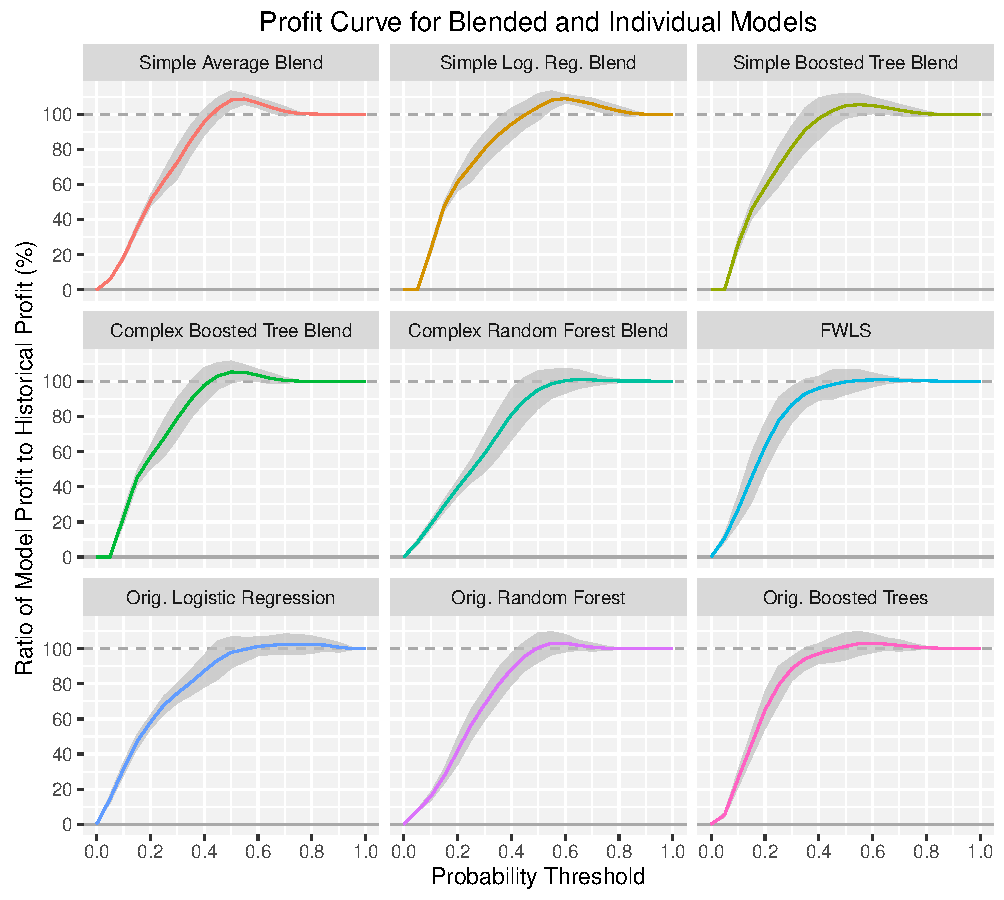
\includegraphics{Consulting_Profitability_Paper_files/figure-latex/profit_curve-1.pdf}
\caption{Profit curves summarising results from 100 models of 9 methods:
3 simple blends, 3 complex blends, and the original 3 best methods.}
\end{figure}

Two blended models clearly outperformed the individual models as shown
in the above plot with higher profit ratios as well as tighter
confidence intervals. The simple Logistic Regression blend performed
best with the highest mean profit ratio of 109\% with a standard
deviation of 1.28\%. \%. This means that for the simple blended Logistic
Regression model, if all jobs above the probability threshold 0.6 were
rejected, the profits would increase on average by 9\% in comparison to
historical profits.

Profit curves from the simple average blend and Logistic Regression
blended models outperformed the complex blended models, which follows
logically from their significantly higher AUC distributions. The simple
average blended model produced a profit curve with an almost identical
profit improvement (and standard deviation) to the Logistic Regression
blend. In the data, projects assigned a probability higher than 0.6
represent only 4.3\% of all projects.

The shaded grey 95\% confidence intervals in the Profit Curve plot shows
that with the 100 sample models that were analysed, none of the lower
bounds for the original methods' or complex blending methods were above
100\% on the y-axis. That is, it cannot be said with 95\% confidence
that the original methods would produce a mean profit higher than
historical profits in the given decision framework. Clearly this level
of certainty is not beneficial for the case-study business to adopt.

It is not clear why simple linear models and the averaging model
outperformed ensemble tree blending methods. As previously stated, the
ensemble trees may not have received enough data to adequately learn the
complex series of rules they develop. The only differences between FWLS
and the simple Logistic Regression (that performed best) were two
additional explanatory variables and four interaction terms. The number
of variables was not high for the amount of data since according to
Peduzzi et al. (1996), 10 events per explanatory variable or more avoids
the risk of biased estimation of variable coefficients in Logistic
Regression. The data contained 315 events per explanatory variable and
did not pose that risk. Nevertheless, the additional variables must have
added misleading noise to the model.

To conclude, because of the promising AUC results, it was logical that
the models translated into financial benefits for the company. The 9\%
improvement in profits produced by the simple blended Logistic
Regression is reasonable, and may be high enough to trigger further
cost-benefit analyses and the development of a more comprehensive
framework describing different decision scenarios.

\begin{itemize}
\item
  decision scenario
\item
  profit curves
\item
  prototype decision support interface
\end{itemize}

\section{6. Conclusions and Future
Work}\label{conclusions-and-future-work}

3/4 page

The general aim was to use statistical techniques to predict the
profitability of projects for a case study consulting business using
their internal CRM data. This was rigorously completed by approaching
the prediction of `profitability' as a binary classification problem
predicting either profit or loss. Several statistical and machine
learning approaches were applied including Naive Bayes, Bayesian
Networks, Linear Regression, Random Forests, gradient Boosted Trees as
well as multiple methods of blending the individual models' output.

AUC = 0.76). This was achieved by 3 individual methods while various
techniques that blended the individual methods improved results further
(AUC = 0.77).

predictive models could be shown to improve the overall profitability
(bottom line) of the case study business. A range of probability
threshold values were trialed for each method using a decision framework
where projects scored below the threshold were accepted, while projects
above the threshold were rejected. If a project was rejected, the
profits and losses were forfeited, and the remaining accepted profits
and losses were summed.

Final results showed the simple Logistic Regression blend of the
individual Logistic Regression, Random Forest and Boosted Tree models
improved profits the most. The 95\% confidence interval for these
improvements was between 6.5\% and 11.5\% using a probability threshold
of 0.6 (approximately 4.3\% of projects).

These results contribute significantly to the research in cost
estimation in three ways: the applied methods, the decision framework,
and the appeal to user trust. Ensemble tree methods and blending had
been applied minimally to cost estimation previously, even though
ensemble trees provide insight into model structure while predicting at
a similar level to Neural Networks. Next, previous studies have verified
predictive accuracy but stopped short of how the algorithm would affect
decisions and what the measured benefits would be. This study presented
a clear framework for how a business could improve profits by applying
the algorithm.

Further work is required to test user confidence in the output. Another
topic identified for future research was to test how well managers
estimate some numeric project input variables. In particular, time span,
team size, total invoiced amount, and percentage of hours completed by
professionals should be tested as these variables were calculated post
project completion. Time span and total invoiced amount were discretised
into wide categories, which should be easier for a manager to choose
between.

future work: user interface.

Overall, this work has successfully built a mathematical blend of
Logistic Regression, Random Forests, and Boosted Tree models, from a
consulting company's internal project data. This blended model can
predict whether a project will be profitable or not and in a reasonable
decision framework, can guide managers in rejecting financially risky
projects and improving profitability of the business.

\section{Acknowledgments}\label{acknowledgments}

This research was supported by a scholarship/ ACEMS?

\section*{References}\label{references}
\addcontentsline{toc}{section}{References}

\paragraph{Installation}\label{installation}

If the document class \emph{elsarticle} is not available on your
computer, you can download and install the system package
\emph{texlive-publishers} (Linux) or install the LaTeX~package
\emph{elsarticle} using the package manager of your TeX~installation,
which is typically TeX~Live or MikTeX.

The author names and affiliations could be formatted in two ways:

\begin{enumerate}
\def\labelenumi{(\arabic{enumi})}
\item
  Group the authors per affiliation.
\item
  Use footnotes to indicate the affiliations.
\end{enumerate}

Bullet points.

\begin{itemize}
\item
  document style
\item
  baselineskip
\item
  front matter
\item
  keywords and MSC codes
\end{itemize}

\hypertarget{refs}{}
\hypertarget{ref-Attalla2003}{}
Attalla, Mohamed, and Tarek Hegazy. 2003. ``Predicting Cost Deviation in
Reconstruction Projects: Artificial Neural Networks Versus Regression.''
Journal Article. \emph{Journal of Construction Engineering and
Management} 129 (4): 405--11.

\hypertarget{ref-Auria2008}{}
Auria, Laura, and Rouslan A Moro. 2008. ``Support Vector Machines (Svm)
as a Technique for Solvency Analysis.'' Journal Article.

\hypertarget{ref-Barber2012}{}
Barber, David. 2012. \emph{Bayesian Reasoning and Machine Learning}.
Book. Cambridge University Press.

\hypertarget{ref-Breiman1996}{}
Breiman, Leo. 1996. ``Bagging Predictors.'' Journal Article.
\emph{Machine Learning} 24 (2): 123--40.

\hypertarget{ref-Breiman2001a}{}
---------. 2001. ``Random Forests.'' Journal Article. \emph{Machine
Learning} 45 (1): 5--32.
doi:\href{https://doi.org/10.1023/A:1010933404324}{10.1023/A:1010933404324}.

\hypertarget{ref-Brown2012}{}
Brown, Iain, and Christophe Mues. 2012. ``An Experimental Comparison of
Classification Algorithms for Imbalanced Credit Scoring Data Sets.''
Journal Article. \emph{Expert Systems with Applications} 39 (3):
3446--53.

\hypertarget{ref-Caruana2006}{}
Caruana, Rich, and Alexandru Niculescu-Mizil. 2006. ``An Empirical
Comparison of Supervised Learning Algorithms.'' Conference Proceedings.
In, 148:161--68. ACM.
doi:\href{https://doi.org/10.1145/1143844.1143865}{10.1145/1143844.1143865}.

\hypertarget{ref-Chan2005}{}
Chan, Swee Lean, and Moonseo Park. 2005. ``Project Cost Estimation Using
Principal Component Regression.'' Journal Article. \emph{Construction
Management and Economics} 23 (3): 295--304.

\hypertarget{ref-Elfaki2014}{}
Elfaki, Abdelrahman Osman, Saleh Alatawi, and Eyad Abushandi. 2014.
``Using Intelligent Techniques in Construction Project Cost Estimation:
10-Year Survey.'' Journal Article. \emph{Advances in Civil Engineering}
2014.

\hypertarget{ref-Elith2008}{}
Elith, Jane, John R Leathwick, and Trevor Hastie. 2008. ``A Working
Guide to Boosted Regression Trees.'' Journal Article. \emph{Journal of
Animal Ecology} 77 (4): 802--13.

\hypertarget{ref-Finnie1997}{}
Finnie, Gavin R, Gerhard E Wittig, and Jean-Marc Desharnais. 1997. ``A
Comparison of Software Effort Estimation Techniques: Using Function
Points with Neural Networks, Case-Based Reasoning and Regression
Models.'' Journal Article. \emph{Journal of Systems and Software} 39
(3): 281--89.

\hypertarget{ref-Flyvbjerg2007}{}
Flyvbjerg, Bent. 2007. ``Cost Overruns and Demand Shortfalls in Urban
Rail and Other Infrastructure.'' Journal Article. \emph{Transportation
Planning and Technology} 30 (1): 9--30.

\hypertarget{ref-Hastie2009}{}
Hastie, Trevor, Robert Tibshirani, and Jerome Friedman. 2009. \emph{The
Elements of Statistical Learning: Data Mining, Inference, and
Prediction, Second Edition}. Book. Springer New York.
\url{http://qut.summon.serialssolutions.com/2.0.0/link/0/eLvHCXMwzV1bS8MwFA7iQBwD3dR6mRAQfNk6trb0Ivi0TQY6EJwgQxi9JLKHddpVf7_nJE269cFnH9NCm_Y7JF--cyPEtnp9s7Im8JCzAWxVjFluEnMWBF4MyyfzE4-HVsR29Tfd9rO89s-BrzBiPSwRH8tocBGfgTxSlGFGrbpQQFAAGIV52JmKxhByhShS_lQg53OGzhsR9IHSKJ6YsfDxcttlP8vYzzrrTEJ4vjYNGaUN8EcoeYfpUofnMCyKACQZ-O6qMEelNAQVpUEpjR1VUGrnKIpucN_BcvnlzqK86ZUNR4cBwrbpes4tFjlf4Yfds9R8fYH9dAA8FGnufK71MnR_ArkqHO7iTW5RQEm_uU4aMEPxsA9subLFFGbHpMYwfaRJ9ljaIkeqaQYt1tAWqU91odzNCXkH0KgCja453QKNKtDuKEJGJWRdqgHrUoCLlnB1qQSLFmCdkpuH8Ww4MXemu_iUBUYW8r_YZ6QRYppDmot0yMQgNQ6myQzkCQZ8l0EO3oKnkT95HMphUw17G5Gz1_vKDaAlwrJNt-edE2pb3PEiL-aRkzh-AKfFqO8nPse2BbFt9S9I-69JXf59-4oclpbTJvt59s2uRQ7tL6t_R8w}.

\hypertarget{ref-Heckerman1998}{}
Heckerman, David. 1998. \emph{A Tutorial on Learning with Bayesian
Networks}. Book. Springer.

\hypertarget{ref-Kim2004}{}
Kim, Gwang-Hee, Sung-Hoon An, and Kyung-In Kang. 2004. ``Comparison of
Construction Cost Estimating Models Based on Regression Analysis, Neural
Networks, and Case-Based Reasoning.'' Journal Article. \emph{Building
and Environment} 39 (10): 1235--42.
doi:\href{https://doi.org/10.1016/j.buildenv.2004.02.013}{10.1016/j.buildenv.2004.02.013}.

\hypertarget{ref-Kragt2009}{}
Kragt, Marit E. 2009. \emph{A Beginners Guide to Bayesian Network
Modelling for Integrated Catchment Management}. Book. Landscape Logic.

\hypertarget{ref-Kumar2007}{}
Kumar, P Ravi, and Vadlamani Ravi. 2007. ``Bankruptcy Prediction in
Banks and Firms via Statistical and Intelligent Techniques--A Review.''
Journal Article. \emph{European Journal of Operational Research} 180
(1): 1--28.

\hypertarget{ref-Louppe2014}{}
Louppe, Gilles, and Peter Prettenhofer. 2014. ``Gradient Boosted
Regression Trees.'' Online Multimedia. PyData.

\hypertarget{ref-Lovallo2003}{}
Lovallo, Dan, and Daniel Kahneman. 2003. ``Delusions of Success: How
Optimism Undermines Executives' Decisions.'' Generic. HARVARD BUSINESS
SCHOOL PUBLISHING CORPORATION.
\url{http://qut.summon.serialssolutions.com/2.0.0/link/0/eLvHCXMw3V3Pb9MwFLYQQxMSEgxYKAPJBwQHlCqO61-TdoC2aNImcdgmcYscxwGktoMlQfvzeXYSJy1M4swxjZuq_uz3vs95PxCi6TSJd2yCAU-T53pmjbIgoblMCqGYyEtpEpoWs-3zt9Bqb_jsfwB-YVdN1Ye3XTS-IaLT_a553GcwEGvXFsO3O1q7kPf3y1trGmf0fDzFouu5U41Za99AKETJb79ROL_-pbtXOIthsZ3pbxvbna-2iexbJww0RKMGq9l5srHVlGS0OsTIBDI-cqakTczcrnO9439CVCCIZQ6ml751Vc_XxXdTn9hNfHUBDhZ4q1cFH5d3utk_feqIVDxwOT5N9Vd24ZnE5RP0uC_pjT-02B2ge3bzFO33k_sMzQOE-LrEHYTHGADEPYB4ABAPAL7DAb7n6OrT8nJ-GnfNLuKvBChkzFTJcgnkVadGg1XkVllKiXYEDHYLYxKUK3imPCfGklIwA8KxYJQpSsAaSHqIHmmXFLGpffJkEaG9EhayjRyriOBfRmj_izpfyNOzeXt50F9OK5_hN_1ZRzC7fh_EfCpeICxEIg2fcebqtoHtzlOic26UYobKWZFMUOQmPXObor7RJiMJT0BSJGqCDnscsmK1yqgrlQfklMBXWlSyH209lQwoEgPdDnfetDCFO2lWpRmoVBDJqRBOq9a3NTxgZ1i_cOABY3jDfSdkYIhgzEueCSL_MmzeFcl3xSHql3f-6BF6OGyaV-h-fdPY1z5t-DdLboxJ}.

\hypertarget{ref-Macdonald1975}{}
Macdonald, P. 1975. ``The Logit Transformation: With Special Reference
to Its Uses in Bio-Assay.'' Journal Article. \emph{Journal of the
Operational Research Society} 25 (1): 201--2.

\hypertarget{ref-Matson1993}{}
Matson, Jack E, and Joseph M Mellichamp. 1993. ``An Object‐oriented Tool
for Function Point Analysis.'' Journal Article. \emph{Expert Systems} 10
(1): 3--14.

\hypertarget{ref-Mendes2004}{}
Mendes, Emilia, and Barbara Kitchenham. 2004. ``Further Comparison of
Cross-Company and Within-Company Effort Estimation Models for Web
Applications.'' Conference Proceedings. In \emph{Software Metrics, 2004.
Proceedings. 10th International Symposium on}, 348--57. IEEE.

\hypertarget{ref-e1071}{}
Meyer, David, Evgenia Dimitriadou, Kurt Hornik, Andreas Weingessel, and
Friedrich Leisch. 2014. \emph{E1071: Misc Functions of the Department of
Statistics (E1071), Tu Wien}.
\url{https://CRAN.R-project.org/package=e1071}.

\hypertarget{ref-Moore1989}{}
Moore, David S, and George P McCabe. 1989. \emph{Introduction to the
Practice of Statistics}. Book. WH Freeman/Times Books/Henry Holt \& Co.

\hypertarget{ref-Pai2013}{}
Pai, Dinesh R., Kevin S. McFall, and Girish H. Subramanian. 2013.
``Software Effort Estimation Using a Neural Network Ensemble.'' Journal
Article. \emph{Journal of Computer Information Systems} 53 (4): 49--58.
\url{http://qut.summon.serialssolutions.com/2.0.0/link/0/eLvHCXMwnV1Nb9QwEB0VekFClPLVAJV8gGPAH4kbc4GlyraIbhftpurRysTe06os3VTqz8fjTbawBanqKZHiOIntvBmPPe8BKPmBpxuYgMHsmgALqtHauDrYJRTaZNlB4b3XiBvxty99pGDV2z1IRuR2PxsKmn8UAUm1IcKwz4tfKclI0XJrp6nxALaJVoSG_Ej-WC8rFHnUE4x_Fmlv_e1WUh7I1fKfFiham-EO9Nuf-tjX_FZywW02x3t_xFN40nmlbLAaRruw5S-ewU6v-MA6AHgOn6bjYXU-mJQs-LfjScXKafVtFMNcjAQ8jtiAnZZnk8FJOFTn48l3Vp5Oy9HXk_IFnA3L6vA47dQX0gWlFaWNwjwjOjfDZ43hssFaovNCu7wIZwpnJrhmuSPtK2xE0QhZ68IJn3PnMzxQL-FxTbv0L9qYzef2gKkw-eJZ1BnFzGcKQ_Ua3SxUyRELTGC_byZbI8V6mnZpbxopgVfr624-t2G-QynmSooE3q-6zy5WLB1W2qW03BYBoSTdrbltr9sE9jbKkaChKLgyCbz7s-PXBWjaGJ6guInGPQFxl2KHHcU6UQu0r__73m_gkYwCG7QB-C08bC-v_H5MOv0NwrD2yw}.

\hypertarget{ref-Peduzzi1996}{}
Peduzzi, Peter, John Concato, Elizabeth Kemper, Theodore R Holford, and
Alvan R Feinstein. 1996. ``A Simulation Study of the Number of Events
Per Variable in Logistic Regression Analysis.'' Journal Article.
\emph{Journal of Clinical Epidemiology} 49 (12): 1373--9.

\hypertarget{ref-Perlich2003}{}
Perlich, Claudia, Foster Provost, and Jeffrey S Simonoff. 2003. ``Tree
Induction Vs. Logistic Regression: A Learning-Curve Analysis.'' Journal
Article. \emph{The Journal of Machine Learning Research} 4: 211--55.

\hypertarget{ref-Provost2013}{}
Provost, F., and T. Fawcett. 2013. \emph{Data Science for Business}.
Book. O'Reilly. \url{https://books.google.com.au/books?id=_1b4nAEACAAJ}.

\hypertarget{ref-gbm}{}
Ridgeway, Greg. 2015. \emph{Gbm: Generalized Boosted Regression Models}.
\url{https://CRAN.R-project.org/package=gbm}.

\hypertarget{ref-Saradhi2011}{}
Saradhi, V Vijaya, and Girish Keshav Palshikar. 2011. ``Employee Churn
Prediction.'' Journal Article. \emph{Expert Systems with Applications}
38 (3): 1999--2006.

\hypertarget{ref-Sealfon2012}{}
Sealfon, Rachel, and Melissa Gymrek. 2012. ``Recitation 6: Random
Forests and Affinity Propagation.'' Online Multimedia. MIT University.
\url{https://stellar.mit.edu/S/course/6/fa12/6.047/courseMaterial/topics/topic4/lectureNotes/recitation6/recitation6.pdf}.

\hypertarget{ref-Shah2014}{}
Shah, Anoop D, Jonathan W Bartlett, James Carpenter, Owen Nicholas, and
Harry Hemingway. 2014. ``Comparison of Random Forest and Parametric
Imputation Models for Imputing Missing Data Using Mice: A Caliber
Study.'' Journal Article. \emph{American Journal of Epidemiology},
kwt312.

\hypertarget{ref-Shin2015}{}
Shin, Y. 2015. ``Application of Boosting Regression Trees to Preliminary
Cost Estimation in Building Construction Projects.'' Journal Article.
\emph{COMPUTATIONAL INTELLIGENCE AND NEUROSCIENCE} 2015: 149702.
doi:\href{https://doi.org/10.1155/2015/149702}{10.1155/2015/149702}.

\hypertarget{ref-Sill2009}{}
Sill, Joseph, Gábor Takács, Lester Mackey, and David Lin. 2009.
``Feature-Weighted Linear Stacking.'' Journal Article. \emph{ArXiv
Preprint ArXiv:0911.0460}.

\hypertarget{ref-Weisberg2005}{}
Weisberg, Sanford. 2005. \emph{Applied Linear Regression}. Book. Vol.
528. John Wiley \& Sons.

\hypertarget{ref-Zhang2004}{}
Zhang, Harry. 2004. ``The Optimality of Naive Bayes.'' Journal Article.
\emph{AA} 1 (2): 3.

\end{document}


